\documentclass[12pt]{report}

\usepackage{circuitikz}
\usepackage{titlesec}
\usepackage{graphicx}
\usepackage{subcaption}
\usepackage{amsmath}
\usepackage{amsfonts}
\usepackage{amssymb}
\usepackage{float}
\usepackage{wrapfig}
\usepackage{booktabs, multirow, soul, changepage, threeparttable}

\graphicspath{{images/}}

\titleformat{\chapter}[display]
{\normalfont\Large\bfseries}{}{0pt}{\Huge \thechapter.\space}
\titlespacing*{\chapter}{0pt}{-20pt}{40pt}


\title{
    \textbf{Constructor University Bremen} \\
    \vspace{1cm}
    \textbf{Lab Report 1: RLC Circuits - Transient Response} \\ 
    Fall Semester 2024 \\
}

\author{
    Author: \textbf{Idriz Pelaj} \\
    \vspace{1cm} \\
    Experiment Conducted By: \\ \textbf{Mr. Idriz Pelaj, Mr. Getuar Rexhepi}
}
\date{Conducted on: \textbf{September 29th, 2023}}

\begin{document}

\maketitle

\chapter{Introduction}
\vspace{-1cm}
In this lab, the Fourier Transform was explored by means of the use of the FFT button on the oscilloscope. The Fourier Transform is a mathematical tool that allows us to convert a signal from the time domain to the frequency domain, thereby allowing the extraction of the frequency components that make up a signal.

A continuous time signal can be described by a sum of sinusoids of different frequencies, amplitudes, and phases. The Fourier Series is a mathematical tool that allows us to decompose a periodic signal into a sum of sinusoids, to use it, however, it must first be established what it means for a signal to be periodic.
We say that a signal is periodic if for some positive period $T$ the following holds:
\begin{equation}
    x(t) = x(t + nT)
\end{equation}
This must hold for all $t$. The fundamental period is the smallest positive period $T$ for which the above holds. The fundamental frequency is defined as:

\begin{equation}
    \omega_0 = \frac{2\pi}{T}
\end{equation}

To determine the complex Fourier Series coefficients, the following equation is used,
\begin{equation}
    c_\nu = \frac{1}{T}\int_{T}f(t)e^{-j\nu\omega_0t}dt
\end{equation}
Where $f(t)$ can then be expressed as,
\begin{equation}
    f(t) = \sum_{\nu=-\infty}^{+\infty}c_\nu e^{j\nu\omega_0t}
\end{equation}
Where the DC component is obtained by substituting $\nu = 0$.
\begin{equation}
    c_0 = \frac{1}{T}\int_{T}f(t)dt
\end{equation}
\newpage
The signal does not have to be represented by complex exponentials, indeed, it can also be represented by sines and cosines, where the fourier coefficients $a_0$, $a_\nu$, and $b_\nu$ are used.
\begin{equation}
    f(t) = \frac{a_0}{2} + \sum_{\nu=1}^{+\infty}a_\nu \cos(\nu\omega_0t) + b_\nu\sin(\nu\omega_0t)
\end{equation}

\section{The Square Wave}
\begin{figure}[H]
    \centering
    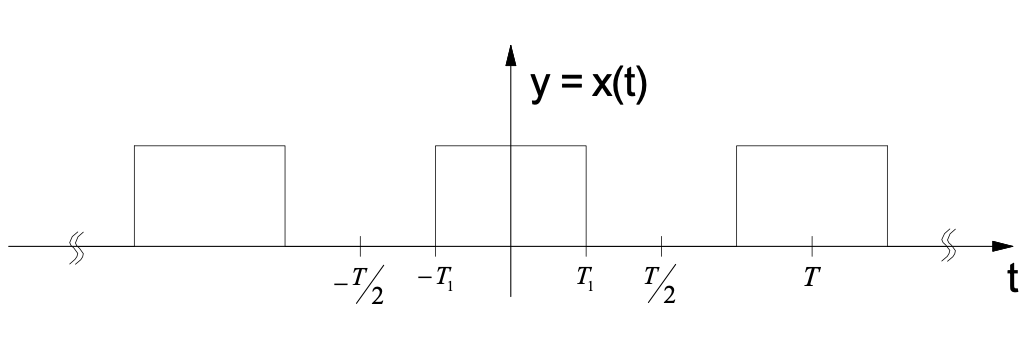
\includegraphics[width=0.8\linewidth]{images/square_wave.png}
    \caption{Square Wave}
    \label{fig:square_wave}
\end{figure}
The square wave shown is a periodic signal that is defined as follows:
\begin{equation}
    x(t) = \begin{cases}
        1 & \text{if } |t| \leq T/2    \\
        0 & \text{if } T_1 < |t| < T/2
    \end{cases}
\end{equation}
Using the equations for the Fourier Series coefficients, and knowing the signal is $1$ between $-T/4$ and $T/4$, and $0$ elsewhere,
\begin{equation}
    c_0 = \frac{1}{T}\int_{-T/2}^{T/2}x(t) dt = \frac{1}{T}\int_{-T/4}^{T/4} 1 dt = \frac{1}{T}\left(\frac{T}{4} - \left(-\frac{T}{4}\right)\right) = \frac{1}{2} \\
\end{equation}
For the $c_\nu$ coefficients,
\begin{equation}
    \begin{gathered}
        c_\nu = \frac{1}{T}\int_{-T_1}^{T_1}x(t)e^{-j \nu\omega_0t} dt \\
        = -\frac{1}{j\nu\omega_0T}e^{-j\nu\omega_0t}\Big|_{-T_1}^{T_1} \\
        = \frac{2}{\nu\omega_0T}\left(\frac{e^{j\nu\omega_0T_1} - e^{-j\nu\omega_0T_1}}{2j}\right)
    \end{gathered}
\end{equation}
Where from Euler's identities, it can be extracted:
\begin{equation}
    c_\nu = \frac{1}{\nu\pi}\sin(\nu\omega_0T_1)
\end{equation}
Where $T$ is the period, and $T_1$ is the width of the pulses.
Similarly, for the $a_\nu$ and $b_\nu$ coefficients extracted from the complex exponential form of the Fourier Series,
\begin{equation}
    a_\nu = 2\Re(c_\nu) = \frac{2}{\nu\pi}\sin\left(\nu\frac{\pi}{2}\right) = \begin{cases}
        0                & {\nu \text{ even}} \\
        \frac{2}{\nu\pi} & {\nu \text{ odd}}
    \end{cases}
\end{equation}
\begin{equation}
    b_\nu = -2\Im(c_\nu) = 0
\end{equation}

Which leads to,
\begin{equation}
    x(t) = \frac{1}{2} + \frac{2}{\pi}\sum_{\nu=1,3,5,...}^{\infty}sin(\nu\frac{\pi}{2})\cdot\frac{cos(\nu\omega_0t)}{\nu}
\end{equation}

The Gibbs Phenomenon is the overshoot of the Fourier Series approximation near the discontinuities of a periodic signal, which most surely can be observed in the case of the square wave. The discontinuities in the pulses makes it necessary to have more and more sinusoids to approximate it, and even then, the approximation is not perfect, leading to "ringing" near the discontinuities.

\begin{figure}[H]
    \centering
    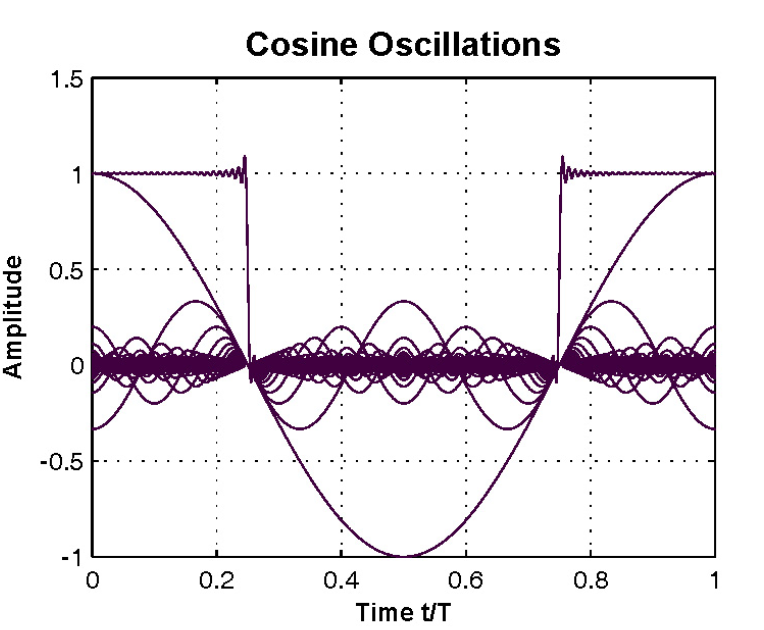
\includegraphics[width=0.8\linewidth]{images/gibbs_phenomenon.png}
    \caption{\centering Gibbs Phenomenon, the overshoot near the discontinuities of the square wave approximated by 50 sinusoids.}
    \label{fig:gibbs_phenomenon}
\end{figure}

\section{The Fourier Transform}

The Continuous Time Fourier Transform is what is obtained when the period of the Fourier Series goes to infinity.
It is defined by,
\begin{equation}
    X(j\omega) = \int_{\infty}^{\infty}x(t)e^{-j\omega t}dt
\end{equation}
And the inverse is given by,
\begin{equation}
    x(t) = \frac{1}{2\pi}\int_{\infty}^{\infty}x(t)e^{j \omega t}d\omega
\end{equation}
For a square pulse, which is essentially a square wave of infinite period, the Fourier Transform is given by,
\begin{equation}
    X(j\omega) = \int_{-\tau/2}^{\tau/2}e^{-j\omega t} dt
\end{equation}

By using Euler's trigonometric identities, it is obtained that the Fourier Transform of the square pulse is given by,
\begin{equation}
    X(j\omega) = \tau \cdot \left[\frac{\sin(\frac{\omega \tau}{2})}{\frac{\omega \tau}{2}}\right] = \tau \cdot sinc\left(\frac{\omega \tau}{2}\right)
\end{equation}

\section{The Discrete Fourier Transform}
Because computers can not handle continuous time signals, an analogous transform to the Fourier Transform is necessary, one that can handle discrete time signals. This is the Discrete Fourier Transform, which is defined as follows:
\begin{equation}
    X[k] = \sum_{n=0}^{N-1}x[n]e^{-j\frac{2\pi kn}{N}}
\end{equation}

And the inverse is given by,
\begin{equation}
    x[k] = \frac{1}{N}\sum_{n=0}^{N-1}X[n]e^{-j\frac{2 \pi kn}{N}}
\end{equation}

\chapter{Execution}
\vspace{-1cm}
\begin{center}
    \begin{tabular}{cc}
        % Left Column (Text)
        \begin{minipage}{0.4\linewidth}
            \begin{itemize}
                \item $V_{pp} = 1\text{V}$
                \item $V_{off} = 0.5\text{V}$
                \item $f = 100\text{Hz}$
                \item $R_i = 50\Omega$
            \end{itemize}
        \end{minipage}
         &
        % Right Column (Circuit)
        \begin{minipage}{0.6\linewidth}
            \begin{circuitikz}
                % Draw a voltage source from 0 to 5V
                \draw (0,0) to [sqV, voltage dir=RP, v=$V_{in}$] (0,4);
                \draw (0,4) to [R, l=$100\Omega$] (\linewidth/4,4);
                \draw (\linewidth/4,4) to [L, l=$10\text{mH}$] (\linewidth/2,4);
                % Draw a C that connects to the voltage in
                \draw (\linewidth/2,4) to [C, l=$6\text{n}8\text{F}$] (\linewidth/2,0);
                \draw (\linewidth/2,0) to (0,0);
            \end{circuitikz}
        \end{minipage}
    \end{tabular}
\end{center}

\begin{enumerate}
    \item The function generator was set to produce a 100Hz square wave with an amplitude of $0.5\text{V}$ and an offset of $0.5\text{V}$. It was checked with the oscilloscope if the signal modulated between $0\text{V}$ and $1\text{V}$.

    \item Subsequently, the R-decade was set to $100\Omega$, and the oscilloscope was connected in parallel to the capacitor.

    \item The damped frequency $f_d$ was measured. To determine $f_d$, the period of the exponentially damped sinusoidal waveform was measured using the oscilloscope. A hardcopy was taken of one signal period and another focusing on the ringing phenomenon.
          \begin{figure}[H]
              \centering
              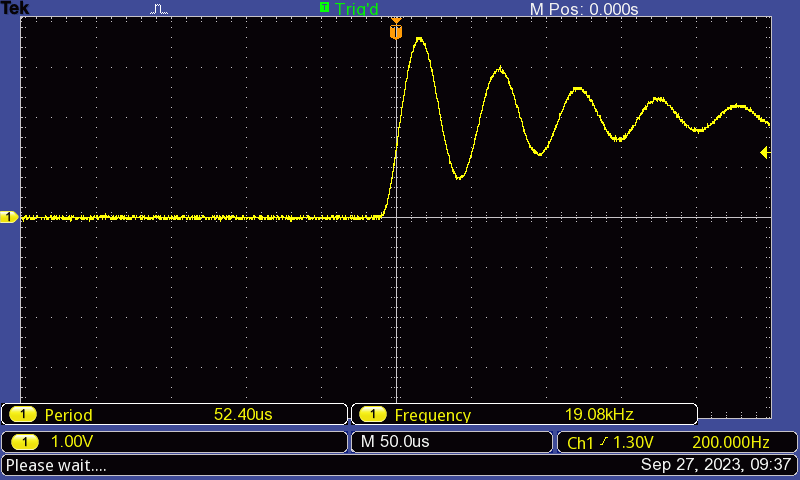
\includegraphics[width=0.8\linewidth]{images/ringing_phenomenon.png}
              \caption{Ringing phenomenon}
              \label{fig:ringing_phenomenon}
          \end{figure}
          According to the figure above, the period of the ringing phenomenon is 52$\mu s$.

    \item Afterward, the damped radian frequency $\omega_d$ was found by knowing that the period of the damped sinusoidal waveform is $f_d = \frac{1}{T}$, where $T=52\mu s$, the period of the ringing phenomenon. Therefore we find that the damped radian frequency $\omega_d$ is
          \begin{equation}
              \begin{gathered}
                  f_d = \frac{1}{T} = \frac{1}{52\mu s} = 1.923 \cdot 10^4 \text{ Hz} \\
                  \omega_d = 2\pi f_d = 1.208 \cdot 10^5 \text{ rad/s}
              \end{gathered}
          \end{equation}
          Very close to the nominal values of
          \begin{equation}
              \begin{gathered}
                  \omega_d = \frac{1}{\sqrt{LC}} = 1.21 \cdot 10^5 \text{ rad/s} \\
                  f_d = \frac{\omega_d}{2\pi} = 1.930 \cdot 10^4 \text{ Hz}
              \end{gathered}
          \end{equation}

    \item The resistance required for the circuit to be critically damped was then calculated.
          \begin{equation}
              \begin{gathered}
                  R = \frac{2\zeta}{\sqrt{C/L}} \implies
                  R_{optimal} = 2\frac{1}{\sqrt{C/L}} - 50\Omega = 2375 \Omega = 2.375 \text{k}\Omega
              \end{gathered}
          \end{equation}
          Where the 50$\Omega$ is subtracted to account for the internal resistance of the function generator.

          \begin{figure}[H]
              \centering
              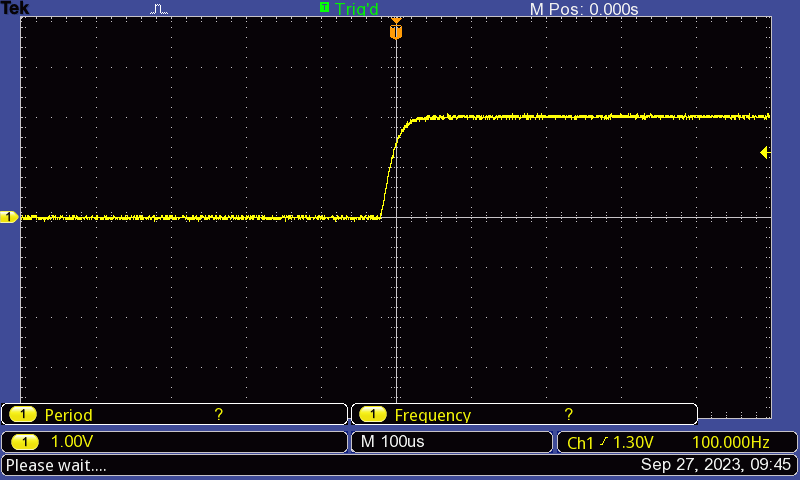
\includegraphics[width=0.8\linewidth]{images/critically_damped_nominal_value.png}
              \caption{Critically damped signal using the nominal resistance value of $2.375\text{k}\Omega$}
              \label{fig:critically_damped_nominal}
          \end{figure}

          However, we find that the optimal resistance is not very close to the nominal value. By playing around with the R-decade, we find that the optimal resistance is
          \begin{equation}
              R_{optimal} = 1905\Omega = 1.905\text{k}\Omega
          \end{equation}

          \begin{figure}[H]
              \centering
              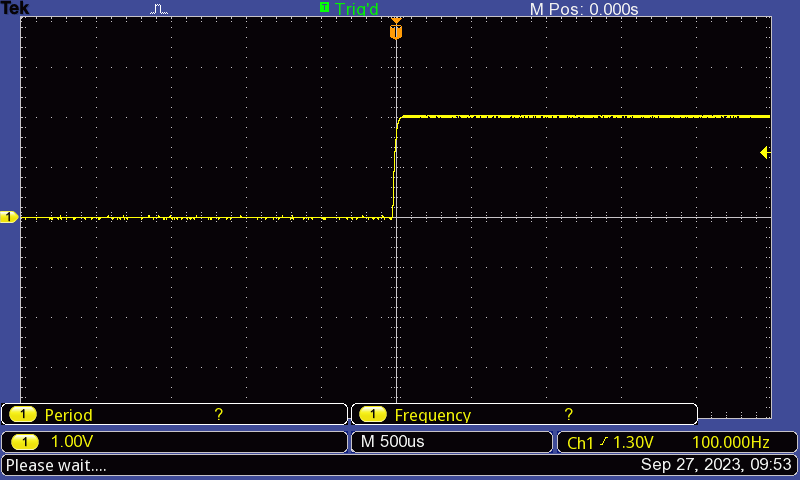
\includegraphics[width=0.6\linewidth]{images/critically_damped.png}
              \caption{Critically damped signal using the tuned resistance value of $1.905\text{k}\Omega$}
              \label{fig:critically_damped_optimal}
          \end{figure}

    \item Finally, the R-decade was set to $30\text{k}\Omega$, causing the circuit to be over-damped. The transient voltage across the capacitor was displayed, and a hardcopy was taken.
          \begin{figure}[H]
              \centering
              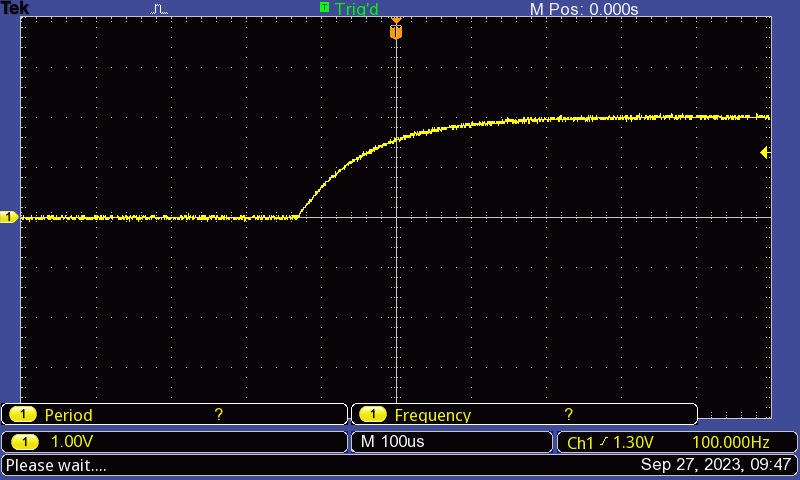
\includegraphics[width=0.6\linewidth]{images/overdamped.png}
              \caption{Over-damped signal}
              \label{fig:over_damped}
          \end{figure}
\end{enumerate}



\chapter{Evaluation}
\vspace{-1cm}
\section{Part 1}
\begin{enumerate}
    \item Based on the experimental observations where when the modulation index was increased the amplitude of the frequency components was increased, and the mathematical theory, it is observed that the amplitude of the relative frequency components grows in relation to the modulation index.

          Mathematically, it is known that the modulation index for an AM signal is given by:
          \begin{equation}
              m = kA_m
          \end{equation}

          Where $k$ is the transmitter sensitivity, and $A_m$ is the modulating signal amplitude, meaning that the modulation amplitude is proportional to the modulation index, while inversely proportional to the transmitter sensitivity.
    \item The modulation index can be computed from the equation found in the prelab, where the modulation index can be found using the maximum amplitude and the minimum amplitude.
          \begin{equation}
              m = \frac{A_{max} - A_{min}}{A_{max} + A_{min}}
          \end{equation}
          For 70\% modulation at the function generator:
          \begin{equation}
              m = \frac{4.32V - 0.8V}{4.32V + 0.8V} \simeq 0.68 \simeq 68\%
          \end{equation}
          For 50\% modulation:
          \begin{equation}
              m = \frac{3.76V - 1.28V}{3.76V + 1.28V} \eqsim 0.49 \eqsim 49\%
          \end{equation}
          For 120\% modulation:
          \begin{equation}
              m = \frac{5.52V + 0.48V}{5.52V - 0.48V} \eqsim 1.19 \eqsim 119\%
          \end{equation}
    \item The disadvantages of using a modulation index greater than 100\% lie in the distortion of the signal, as the carrier wave is not able to fully represent the modulating signal, therefore the envelope of the signal is distorted, making the signal unrecoverable.
\end{enumerate}

\section{Part 2}
\begin{enumerate}
    \item The spectrum in the oscilloscope for the 70\% modulation is shown to be 20KHz for the carrier wave, and 19.81KHz for the modulating wave. When plotting the FFT of the signal in theory using MATLAB, similar results are observed:
          \begin{figure}[H]
              \centering
              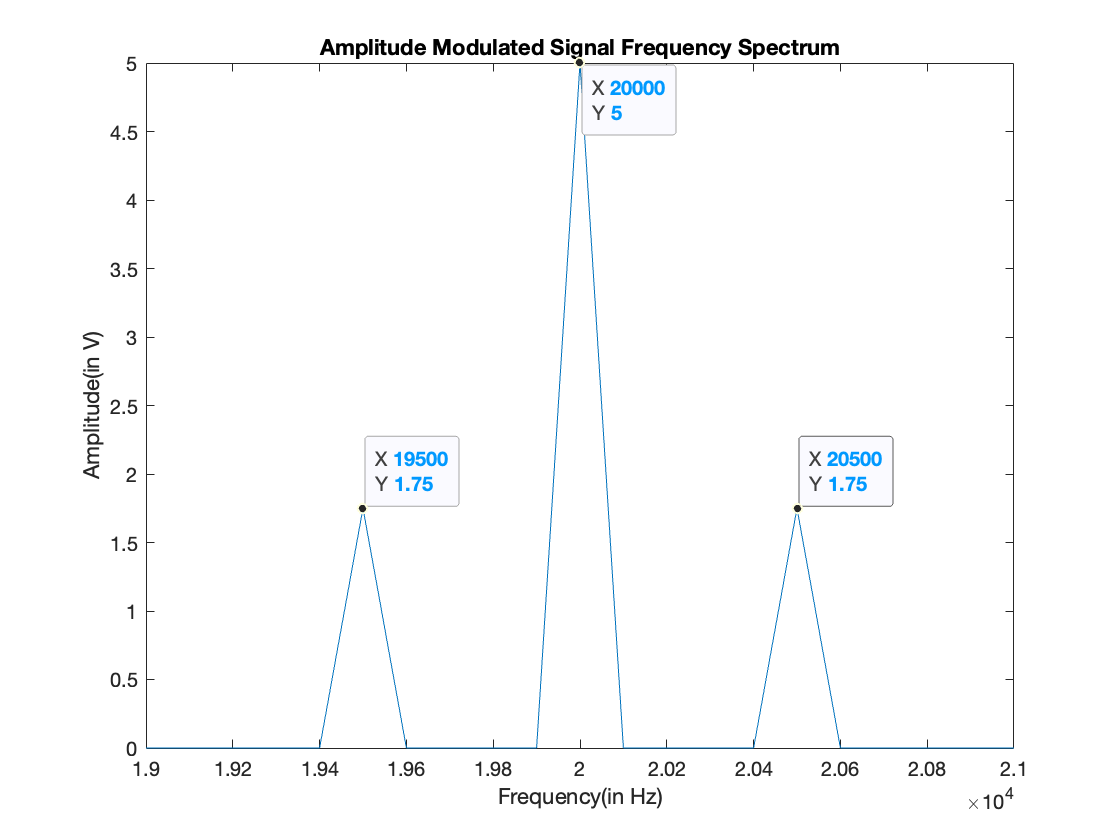
\includegraphics[width=0.5\textwidth]{images/evaluation_part2.png}
              \label{fig:evaluation_part2}
              \caption{Theoretical 70\% modulation index FFT, with the peaks at 19.5KHz, 20KHz, and 20.5KHz respectively}
          \end{figure}
    \item The function generator clearly generates a double-sideband signal, without suppressing the carrier as the carrier is observed in the fourier transform of the signal in the oscilloscope.
    \item When changing the carrier frequency of the signal, the spacing of the sidebands changes to move accordingly, as the modulating signal is convolved with the carrier signal.
    \item Changing the message frequency of the signal changes the width of the spectrum of the signal, as the modulating signal is convolved with the carrier signal and the width of the sidebands changes.
    \item The modulation index in the frequency spectrum can be found by taking the ratio between one of the sideband peaks amplitudes and the carrier peak amplitudes, so
          \begin{equation}
              m = \frac{4.15dB}{5.05dB} \simeq 0.82 \simeq 82\%
          \end{equation}
          This implies that the FFT of the signal as measured on the oscilloscope is not a perfect representation of the signal, as the modulation index is not 70\% as expected.
\end{enumerate}

\section{Part 3}
\begin{enumerate}
    \item The first order and the third order message signal as displayed in the oscilloscope show that the envelope of the signal is tracked better by the third order filter, with the first order filter not being able to track the amplitude peaks in order to track the envelope of the signal in the same manner.
    \item The first order filter is quite similar to what is observed in MATLAB, with the first order filter not being able to track the envelope of the signal with the same accuracy as the third order filter. The differences between the measurement and the simulation are due to the fact that the simulation is done using an ideal filter, while the measurement is done using a real filter, which has a non-ideal frequency response.
\end{enumerate}


\chapter{Conclusion}
\vspace{-1cm}
The behavior of AM modulation was explored via the use of the function generator's ability to generate AM signals, and the behaviour was observed using the oscilloscope. Furthermore, a slope detection circuit was assembled on the breadboard in order to demodulate the AM signal. The difference between first and third order slope detection was observed. The FFT of the oscilloscope's resolution, in part, causes the error in trying to observe the frequency peaks and finding the true modulation index in the case of 70\% modulation provided by the function generator, where it was obtained from the determined frequency that it was 82\%. Artifacts in the de-modulated signal are due to the internal resistance of the inductors, capacitors, and also due to the other components not being ideal. The wires have their own resistance as well. Overmodulation was also observed, and the effect it has on the envelope of the signal.

\chapter{References}
\vspace{-1cm}
\begin{enumerate}
    \item Oscilloscope Manual
    \item Lab Manual for Signals and Systems
    \item MATLAB Documentation
\end{enumerate}

\chapter{Appendix}
\vspace{-1cm}
\section{Prelab Code:}
\begin{verbatim}
%% Prelab:

% Prelab Problem 2:
Fs = 1e5;
t = 0:1/Fs:0.01;
f = 20E3; % 20 Khz

A_c = 5;

f_m = 5E2;
x = sin(2*pi*f_m*t);

f_c = 20E3;
y = A_c*(1+0.5*x).*cos(2*pi*f_c*t);

subplot(3, 2, 1);
plot(t, x);
title('Modulating Signal');
xlabel('Time(in s)');
ylabel('Voltage(in V)');

subplot(3, 2, 2);
plot(t, y);
title('Amplitude Modulated Signal');
xlabel('Time (in s)');
ylabel('Voltage (in V)');

% Frequency spectrum

N = length(y);
Y = fft(y);

spectrum = abs(Y/N);
spectrum_single = spectrum(1:N/2+1);
spectrum_single(1:end-1) = 2*spectrum_single(1:end-1);

F = Fs * (0:(N/2)) / N;
subplot(3, 2, 3);
plot(F, spectrum_single);
xlim([1E3, 5E4]);
title('Amplitude Modulated Signal Frequency Spectrum');

frequencies = logspace(3, 5, 100); % 100 Hz to 100 KHz
Wn = 1000/(f/2); % Normalized cutoff frequency

[b1, a1] = butter(1,Wn); % Butterworth filter of first order
[b3, a3] = butter(3, Wn); % Butterworth filter of third order

% Rectify the signal

% We can use an envelope detector for this, the simplest analogue to a
% diode would be the absolute value of the signal, so that's what will be
% used

rectified = abs(y);
filtered = filter(b1, a1, rectified);

% figure;
subplot(3, 2, 4);
plot(t, rectified);
title('First-Order Demodulated Signal');
xlabel('Time(in s)');
ylabel('Voltage(in V)');

filtered3 = filter(b3, a3, rectified);
subplot(3, 2, 5);
plot(t, filtered3);
title('Third-Order Demodulated Signal');
xlabel('Time(in s)');
ylabel('Voltage(in V)');

% Bode plot for the filters
figure;
freqs(b1, a1);
title("First Order Butterworth Filter Bode Plot");

figure;
freqs(b3, a3);
title("Third Order Butterworth Filter Bode Plot");
\end{verbatim}

\end{document}